\section{Preliminary Study}

\begin{figure}[!t]

  \centering
  \hspace*{-1em}

  \begin{minipage}{4in}
    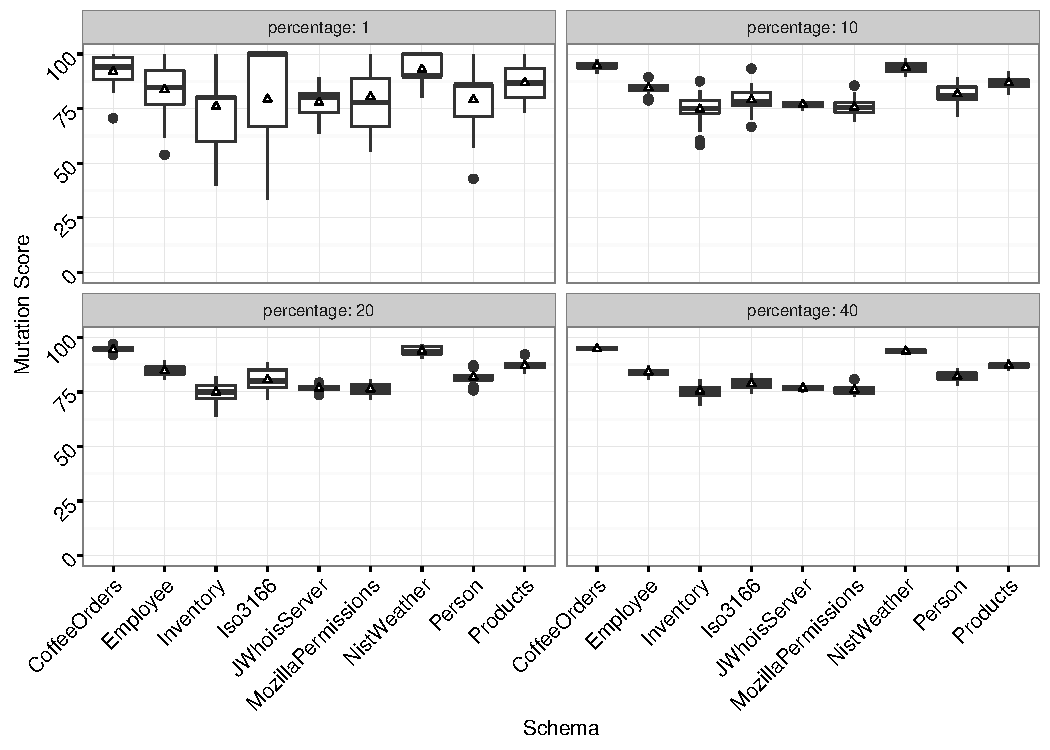
\includegraphics[scale = 0.5]{graphs/schema_vs_ms.pdf}
  \end{minipage}

  \caption{\label{fig:graph}Graph displaying mutation scores for database schemas.}

  \vspace{-1.8em}

\end{figure}


% GMK NOTE: All of this content is really about the design of the experiments and thus it has to be integrated into this
% section (currently, this is still rough content).

To display the effectiveness and the domain extensibility of \mr, we empirically analysed the nine schemas in Table~\ref{tbl:study-schemas}
with the presented tool. These schemas were chosen due to the range in triviality --- the total number of constraints ({\small$\sum$Constraints}).
This range in triviality allowed us to evaluate the effectiveness of reduction techniques performed by \mr~for schemas of varying
complexities.

Similar to Wong and Mathur in their studies~\cite{mathur1994empirical, wong1993mutation} where they conducted experiments using
mutant sampling with $x$ values ranging from $10\%$ to $40\%$, increasing by steps of $5\%$, we chose to analyse $x$ at $1\%$ and
then increase by $10\%$ intervals up to $90\%$. By lowering the granularity of the experiment to $10\%$ intervals instead of $1\%$
or $5\%$, \mr~reduces the cost of performing retrospective analysis, while observing similar trends, which are displayed in
Figure ~\ref{fig:graph}.

% CJM: to find the distance between original and reduced mutation scores
% this example below is just for an x value of 1 and for random sampling

% d <- read_data("sqlite-avmdefaults.dat")
% d <- select_empirical_study_schemas(d)
% d <- select_normal_data(d)
% t <- analyse(d)
% t_filt <- dplyr::filter(t, method == "random_sampling", percentage == 1)
% diff <- abs((t_filt$original_mutation_score - t_filt$reduced_mutation_score))
% max(diff)
% [1] 0.4666667

% CJM: to find the min and max RMSE at a given percentage
% this example below is just for an x value of 1 and for random sampling

% d <- read_data("sqlite-avmdefaults.dat")
% d <- select_empirical_study_schemas(d)
% d <- select_normal_data(d)
% t <- analyse(d)
% t_filt <- dplyr::filter(t, method == "random_sampling", percentage == 1)
% c <- analyse_calculations(t_filt)
% max(c$root_mean_squared_error)
% [1] 0.20367
% min(c$root_mean_squared_error)
% [1] 0.06175125

% CJM: to create the visualisation currently in the paper:

% d <- read_data("sqlite-avmdefaults.dat")
% d <- select_empirical_study_schemas(d)
% d <- select_normal_data(d)
% t <- analyse(d)
% pers <- c(1, 10, 20, 40)
% t_filt <- dplyr::filter(t, method == "random_sampling", percentage %in% pers)
% visualise_mutation_score_across_schemas(t_filt)

Figure~\ref{fig:graph} is a box-and-whisker plot displaying the analysed schemas from Table~\ref{tbl:study-schemas} on the horizontal-axis
and on the vertical-axis, the mutation scores of the reduced sets after random sampling at the following $x$ values: 1\%, 10\%, 20\%, 40\%.
In Figure~\ref{fig:graph}, the $x$ values were chosen in this range because the reduced set's mutation scores at these thresholds
drastically increase in accuracy --- approach the mutation score of the original set. Moving from top-left to bottom-right, the boxes in
Figure~\ref{fig:graph} show this increase in accuracy by becoming smaller as the maximum fractional threshold increases.

This increase in accuracy occurs because the mutation scores of reduced sets with smaller fractional thresholds are extremely volatile
and can vary largely based on one or a few mutants, while the mutation scores of sets with higher fractional thresholds are substantially
more stable. In the top-left of Figure~\ref{fig:graph}, $x$ is set to 1\%. At 1\% the sets' mutation scores are as volatile as possible,
being as distant from the original mutation as $0.467$. Additionally, at this maximum fractional threshold, the ``lower-is-better'' metric,
RMSE, ranges from $0.062$ to $0.204$. Stability is demonstrated in mutation scores of sets with as small as a 10\% maximum fractional
threshold, with RMSE ranging from $0.013$ to $0.065$. At this same maximum fractional threshold, Wong and Mathur observed that the mutation
scores of reduced sets were within $0.16$ of the original set's mutation score~\cite{mathur1994empirical, wong1993mutation}. Using \mr~to
retrospectively perform random sampling with an $x$ value of 10\%, we observed mutation scores of reduced sets to be within $0.13$ of the
original set's mutation score.

The trend of becoming more accurate as the maximum fractional threshold increases remains true for $x$ values of 20\% and 40\%. At maximum
fractional thresholds of 20\% and 40\%, the mutation scores of reduced sets are within $0.083$ and $0.075$ of the original mutation scores,
respectively. It is acknowledged that the results experienced in the preliminary study of \mr~may be specific to the sample data used or
database schemas being the domain analysed.
